% K3-only adaptation of the author's approved vector schematic.
% Block sizes indicate functional grouping, not measured runtime.
\documentclass[10pt,border=0pt]{standalone}
\usepackage{fontspec}
\setmainfont{Times New Roman}
% 9.134125 TeX pt = 9.1 PDF pt; natural canvas width is 60 mm.
\newcommand{\FigureFont}{\fontsize{9.134125}{11}\selectfont}
\usepackage{tikz}
\definecolor{kernelblue}{HTML}{4E79A3}
\newcommand{\Stage}[3]{%
  \draw[fill=kernelblue,draw=black,line width=.90pt] (.10,#1) rectangle (.66,#2);
  \draw[fusionbracket] (.75,{#1+.035}) -- (.82,{#1+.035}) -- (.82,{#2-.035}) -- (.75,{#2-.035});
  \node[anchor=west,inner sep=0pt,font=\FigureFont] at (.94,{(#1+#2)/2}) {#3};
}
\begin{document}
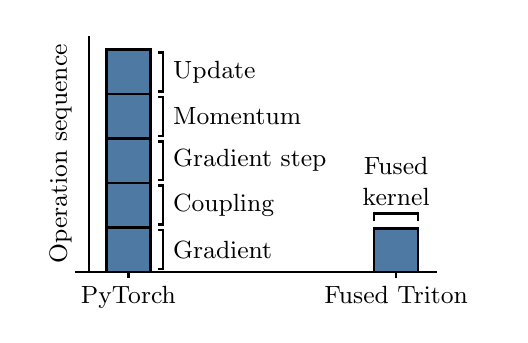
\begin{tikzpicture}[x=1cm,y=1cm,text=black,
  fusionbracket/.style={draw=black,line width=.90pt,line cap=butt,line join=miter}]
  \useasboundingbox (-.90,-.55) rectangle (5.10,3.10);
  \draw[black,line width=.90pt] (-.30,0) -- (4.30,0);
  \draw[black,line width=.90pt] (-.12,0) -- (-.12,3.00);
  \node[rotate=90,font=\FigureFont,inner sep=0pt] at (-.48,1.50) {Operation sequence};
  \draw[black,line width=.90pt] (.38,0) -- (.38,-.075);
  \draw[black,line width=.90pt] (3.78,0) -- (3.78,-.075);
  \draw[fill=kernelblue,draw=black,line width=.90pt] (3.50,0) rectangle (4.06,.55);
  \draw[fusionbracket] (3.50,.65) -- (3.50,.74) -- (4.06,.74) -- (4.06,.65);
  \node[font=\FigureFont,align=center,anchor=south,inner sep=0pt] at (3.78,.84) {Fused\\kernel};
  \node[font=\FigureFont,anchor=north,inner sep=0pt] at (.38,-.17) {PyTorch};
  \node[font=\FigureFont,anchor=north,inner sep=0pt] at (3.78,-.17) {Fused Triton};
  \Stage{0}{.564}{Gradient}
  \Stage{.564}{1.128}{Coupling}
  \Stage{1.128}{1.692}{Gradient step}
  \Stage{1.692}{2.256}{Momentum}
  \Stage{2.256}{2.82}{Update}
\end{tikzpicture}
\end{document}
